\section{Parallel computing in GPU}
TODO: fiks på dette
A huge disadvantage with the level set method for segmentation is that it is very slow when working with big data volumes in 3D space. Implementations of level set algorithms for 3D in the graphical processing unit (GPU) parallelizes the level set method and makes it much faster. One of the first GPU based 3D implementations of the level set method was by Lefohn et al. in \cite{cates03} in 2003. In this paper a modified sparse field level set method was implemented for the GPU using graphic APIs such as OpenGL and DirectX. In the past few years general purpose GPUs have made implementing level set methods and other non-graphical tasks in GPUs much easier. In \cite{panlei08} some simple medical segmentation algorithms was implemented using NVIDIAs CUDA technology, and in \cite{Packer10} CUDA was used to implement the level set method.


\subsection{Data and task parallelism}
Data and task parallelism are the two main categories of computer parallelism. Data parallelism is achieved by having differnt units execute the same task at different data in parallel. This type of parallelism is used in image processing where for example all pixels are increased by the same value. 
When using task parallelism the tasks are seperated to different executional units (usually cores) and executed on different data. Task parallelism is seperated into two parts based on the type of communication used between the executional units. These two methods are the shared memory method, and the message passing method used in distributed memory. When using shared memory the executional units have a shared space in the memory that all executional units can read from and write to. To control that no conflicts arises when multiple units accesses the shared memory locks have to be used. By using locks the part in memory that a unit is writing to cannot be accessed by any other unit, and only when a unit is finished writing is the lock released to provide other units access to the memory data or the lock. Synchronization to prevent race conditions (occurs when operations depending on each other is executed in the wrong order) so that a unit does not change the value of a memory location before other units have used it is also an important factor when using shared memory. Pthreads is an API that supports shared memory multiprocessing, and another which will be introduced later in this chapter is OpenMP. The other method for communication between the units is message passing which is used in distributed memory systems such as supercomputers. The communication is handled by sending and receiving messages between the units. Messages sent can be one of several different types, such as synchronous or asynchronous, one-to-one or one-to-many. Several message passing systems exists, some of them being the Java Remote Method Invocation, Simple Object Access Protocol (SOAP) and the popular Message Passing Interface (MPI). 

\subsection{Central processing unit}
The central processing unit (CPU) .....

\subsection{Flynn's taxonomy of computer architectures}
Michael J. Flynn proposed in 1996 a taxonomy of classification of computer architectures. Taxonomy is the study of the general principles of scientific classification. Flynn described four different types based on the use use of one or multiple numbers of data and instructions.
 
\subsubsection*{Single Instruction Single Data - SISD}
The SISD architecture uses no parallelism in either the data stream or the instruction stream. SISD is used in uniprocessors and exectues a single instruction on a single data. Figure \ref{SISD} illustrates how SISD works. In the figure processing unit is abbreviated as PU.
\begin{figure}[h!]
\centering
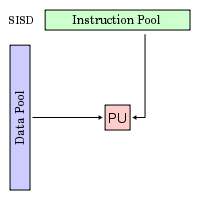
\includegraphics[width=0.50\textwidth]{backgroundTheory/parallel/SISD}
\caption{Single Instruction Single Data.}
\label{SISD}
\end{figure}

\subsubsection*{Single Instruction Multiple Data - SIMD}
Architectures based on SIMD uses  multiple processing units to execute a single instruction on multiple data. Thus SIMD uses data level parallelism as previously discussed. Modern CPUs are all able to perform SIMD instructions and they are able to load n numbers (n may vary depending on design) of data to memory at once and and execute the single instruction on the data. An example where SIMD instrctions can be used is in image preocessing where several pixels are to be added or subtracted the by samme value. How SIMD instructions works is shown in figure \ref{SIMD}
\begin{figure}[h!]
\centering
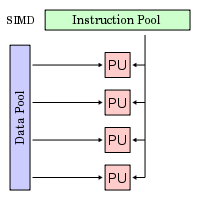
\includegraphics[width=0.50\textwidth]{backgroundTheory/parallel/SIMD}
\caption{Single Instruction Multiple Data.}
\label{SIMD}
\end{figure}

\subsubsection*{Multiple Instruction Single Data - MISD}
MISD is the least used archetecture type of the four in Flynn's taxonomy. This is because doing multiple instructions on a single data is much less scalable and it does not utilize computational resources as good as the rest. MISD is illustrated in figure \ref{MISD}.
\begin{figure}[h!]
\centering
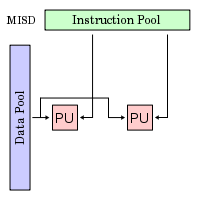
\includegraphics[width=0.50\textwidth]{backgroundTheory/parallel/MISD}
\caption{Multiple Instruction Single Data.}
\label{MISD}
\end{figure}

\subsubsection*{Multiple Instruction Multiple Data - MIMD}
Being able to do multiple instructions on multiple data is possible by having different processors execute instructions on multiple data. Modern CPUs consisting of several cores are all based on MIMD for parallelism. MIMD is illustrated in figure \ref{MIMD}.
\begin{figure}[h!]
\centering
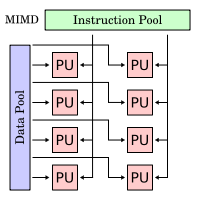
\includegraphics[width=0.50\textwidth]{backgroundTheory/parallel/MIMD}
\caption{Multiple Instruction Multiple Data.}
\label{MIMD}
\end{figure}

\subsection{Graphics processing unit}
A graphics processing unit (GPU) is a specialized chip that initially was designed to offload the CPU and accelerate processes associated with computer graphics. The process of computing the color of each pixel on screen is memory intensive but independent of each other and thus highly parallelizable. 

\subsection{OpenMP}
OpenMP is an API that supports shared memory parallel programming in C, C++, and Fortran for multiple processor architecture types and operative systems. OpenMP was designed to allow programmers to incrementally parallelize existing serial programs, which is difficult with MPI and Pthreads \cite{peter11}. OpemMP makes it simple to code parallel behaviour by allowing the compiler and run-time system to determine some of the thread behaviours details. OpenMP is a directive based API, which means that a a serial code can be paralellized with little effort and a carefully written OpenMP program can be compiled and run as a serial program if the compiler does not support OpenMP. 

\subsection{General Purpose GPU}
TODO 

\subsection{CUDA}
CUDA (Compute Unified Device Architecture) is a program development environment introduced by NVIDIA in 2006 for their GPUs in C/C++ and Fortran\cite{cudaWebpage}. CUDA and OpenCL (which unlike CUDA supports all kinds of GPUs) have made GPU programming much more user-friendly than before, when the tasks had to be transformed into rendering problems. CUDA programs are initialized on the CPU (called the host) and then the data needed for the computation in the GPU (called the device) is initialized in the CPU and copied over the PCI bus to the GPU. When the computation is finished, the results are copied back to the CPU. In CUDA, a kernel is a program (function) that is executed in the device. The kernel code is run in parallel on a number of threads. Threads are grouped into blocks whose size (number of threads in a block) and dimension (up to 3D) can be decided by the programmer, within the maximum limit of 1024 threads per block (for compute capability of 2.0 or higher). But 32 threads will always execute the same code (even if less than 32 executions is needed), and such a group of 32 threads is called a warp. Thus, the number of blocks used should be a multiplum of the warpsize to achieve maximum performance. It must be noted that warps are not a part of the CUDA model but device dependent, and even though the warpsize usually is 32, it does vary from device to device. Figure \ref{CUDAProgModel} illustrates the programming model of CUDA, which also shows that a set of blocks is called a grid.

\begin{figure}[h!]
\centering
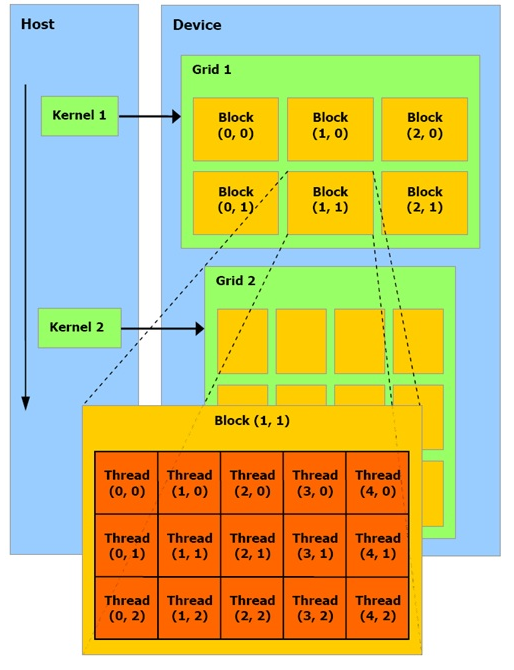
\includegraphics[width=0.65\textwidth]{backgroundTheory/parallel/CUDAProgModel}
\caption{CUDA programming model.}
\label{CUDAProgModel}
\end{figure} 

Each thread in CUDA have its own registers and local memory, and all the threads in a block have a shared memory, all which can be written to and read from the device. In addition all threads in a grid share global, constant and texture memory which can be read and written by the host and the device (constant and texture memory is read-only for the device). How these are connected together is indicated in figure \ref{CUDAMemModel}. Registers are the smallest, but also the fastest, and the per-thread register limit for compute capability (version) 3.0 is 63 registers per thread. If a thread needs more than 63 registers the shared memory is used (L1 cache) which is much slower. And if even more is needed the even slower global is also used.

\begin{figure}[h!]
\centering
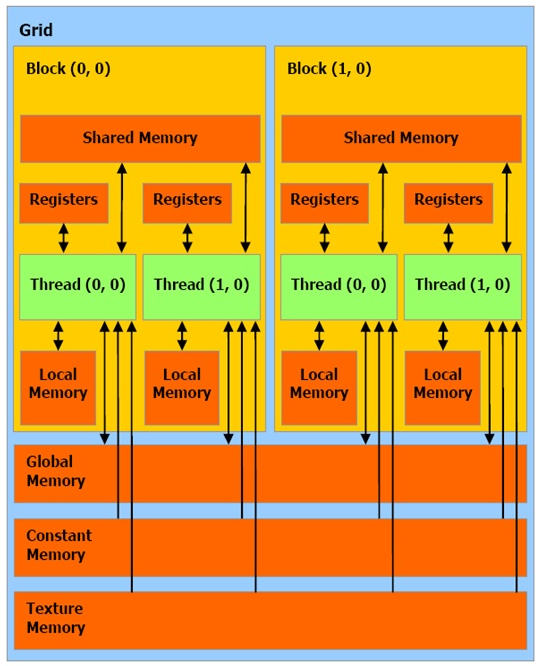
\includegraphics[width=0.90\textwidth]{backgroundTheory/parallel/CUDAMemModel}
\caption{CUDA memory model.}
\label{CUDAMemModel}
\end{figure} 

Functions used in CUDA code can be of different types. A global function (with the identifier \_\_global\_\_ in front) is a function that runs on the device, but only callable from the host. The second type is device (\_\_device\_\_), and this type of functions are only callable by functions running on the device, i.e. device and global functions. The last type, host, is code that only runs on the host. Host functions can be identified by the syntax \_\_host\_\_ in front of the return type, but this is not required. NVIDIAs own compiler, nvcc, splits up the code into host and device components, compiles the global and device functions itself, and lets the standard host compiler compile the host code. If the same functions is needed in both host and device it can be compiled as by both nvcc and the host compiler if it is identified by both \_\_host\_\_ and \_\_device\_\_.  The syntax for calling a kernel from the device is kernelName$<<<$numBlocks, numThreadsPerBlock$>>>$(arg1, arg2, ..., argN). The triple angle brackets indicate that it is a kernel launch. The first number within these brackets is dimension of the grid, measured in the number of blocks in that grid. The second is the block dimension, i.e. the numbers of threads in a block. Calling a kernel with $X$ number of blocks and $Y$ number of threads per block results in $X*Y$ parallel executions of that kernel. 

Algorithm \ref{CUDAex} (from \cite{jason10}) is a simple CUDA program in C++ that shows the basic CUDA syntax. In line 4 three arrays are created, and in line 5 copies of these to be used in the device is created. These have to be pointers (even if they are not arrays as in this case) because they are to be used on the device and must point to device memory. In line 9-11 space is allocated for the arrays using cudaMalloc in the device just like calling malloc would allocate space on the host. After two of the arrays have been filled with random values they are copied over to the device using the cudaMemcpy function in line 22-23. The cudaMemcpy function takes in four inputs. The first input is the destination address, which in this case was allocated in line 9-10, the second input is the source to copy, the third input is the size in bytes and the last input is the type of transfer. Type of transfer is either cudaMemcpyHostToDevice or cudaMemcpyDeviceToHost indicating transfer from host to device and device to host, respectively. On line 26 the kernel is launched. The code within the kernel (line 38-43) is written as serial code, and to differentiate between the different threads all threads can be assigned an unique thread identification. This thread-id is calculated as the id of the thread within the block (threadIdx), plus the id of the block (blockIdx) times the number of blocks (blockDim). The if-sentence in line 40 avoid errors in case the size of the array is less than the number of threads started (not necessary in this case since the number of threads is equal to the array size). Inside the if-sentence each thread does one addition with its thread-id as the position in the arrays.  At line 29 the result array is copied back to the CPU, and lastly the allocated space in the GPU is freed in line 32-34.

\lstinputlisting[caption={Simple CUDA program}, label={CUDAex}, numbers=left, belowcaptionskip=4pt]{backgroundTheory/parallel/CUDAexampleCode.c} %inputs the source code with numbered lines
















